\documentclass{article}
\usepackage[T1]{fontenc}
\usepackage[utf8]{inputenc}
\usepackage{lmodern}
\usepackage[tmargin=0.75in,lmargin=0.75in,rmargin=0.75in]{geometry}
\usepackage{subcaption}
\usepackage{graphicx}
\usepackage{subcaption}


\begin{document}
\renewcommand{\baselinestretch}{1.0}
\begin{center}
\Large{\textbf{FastQC Quality Results}}
\end{center}
\section{Basic Statistics}
\begin{description}
\renewcommand{\baselinestretch}{1.0}
\item[Filename:]
04{-}R1.qfilter.fastq.gz
\item[File type:]
Conventional base calls
\item[Encoding:]
Sanger / Illumina 1.9
\item[Total Sequences:]
310338
\item[Sequences flagged as poor quality:]
0
\item[Sequence length:]
50{-}150
\item[\%GC:]
40
\end{description}


\section{Graphs}
\begin{description}
\item[Overrepresented sequences:]
None
\end{description}


\begin{figure}[htbp]
\centering
\begin{subfigure}{0.45\linewidth}
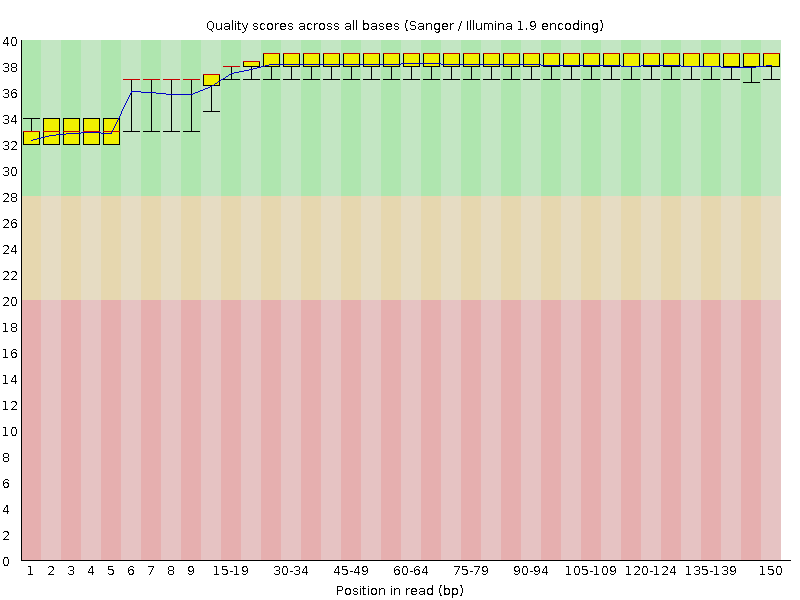
\includegraphics[width=\linewidth]{04-R1.qfilter_fastqc/Images/per_base_quality.png}
\caption{Per base sequence quality: PASS}
\end{subfigure}
\begin{subfigure}{0.45\linewidth}
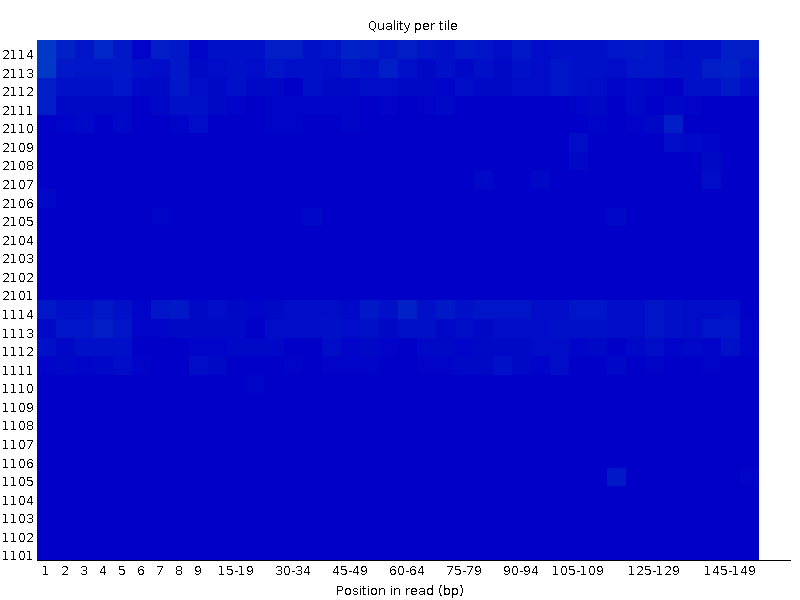
\includegraphics[width=\linewidth]{04-R1.qfilter_fastqc/Images/per_tile_quality.png}
\caption{Per tile sequence quality: PASS}
\end{subfigure}
\begin{subfigure}{0.45\linewidth}
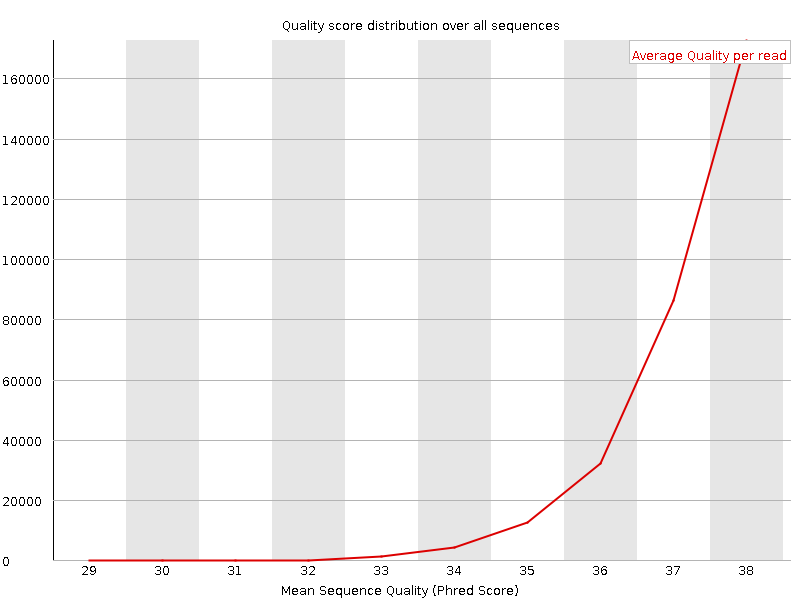
\includegraphics[width=\linewidth]{04-R1.qfilter_fastqc/Images/per_sequence_quality.png}
\caption{Per sequence quality scores: PASS}
\end{subfigure}
\begin{subfigure}{0.45\linewidth}
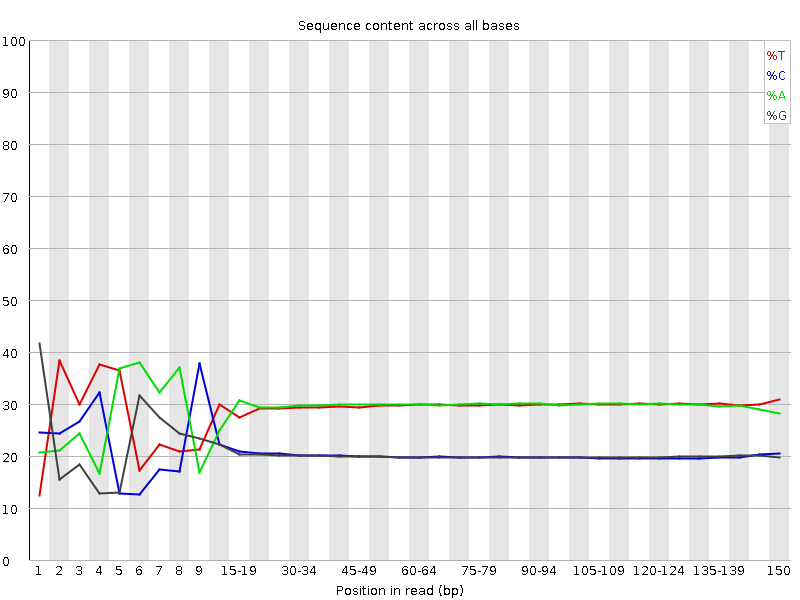
\includegraphics[width=\linewidth]{04-R1.qfilter_fastqc/Images/per_base_sequence_content.png}
\caption{Per base sequence content: FAIL}
\end{subfigure}
\end{figure}




\begin{figure}[htbp]
\ContinuedFloat
\centering
\begin{subfigure}{0.45\linewidth}
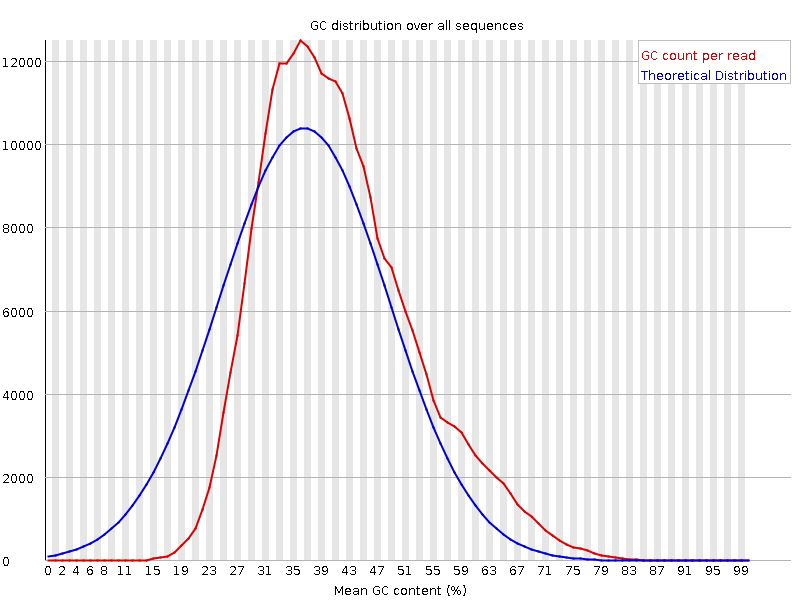
\includegraphics[width=\linewidth]{04-R1.qfilter_fastqc/Images/per_sequence_gc_content.png}
\caption{Per sequence GC content: FAIL}
\end{subfigure}
\begin{subfigure}{0.45\linewidth}
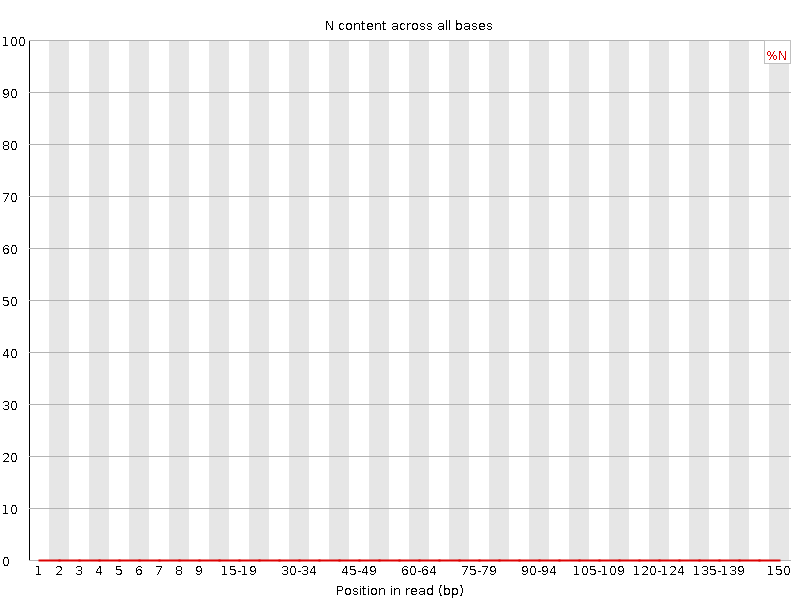
\includegraphics[width=\linewidth]{04-R1.qfilter_fastqc/Images/per_base_n_content.png}
\caption{Per base N content: PASS}
\end{subfigure}
\begin{subfigure}{0.45\linewidth}
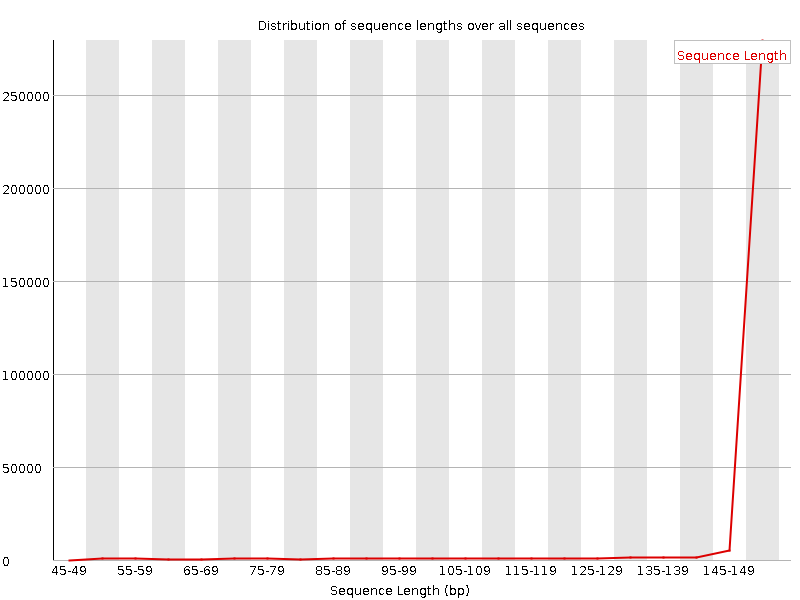
\includegraphics[width=\linewidth]{04-R1.qfilter_fastqc/Images/sequence_length_distribution.png}
\caption{Sequence Length Distribution: WARN}
\end{subfigure}
\begin{subfigure}{0.45\linewidth}
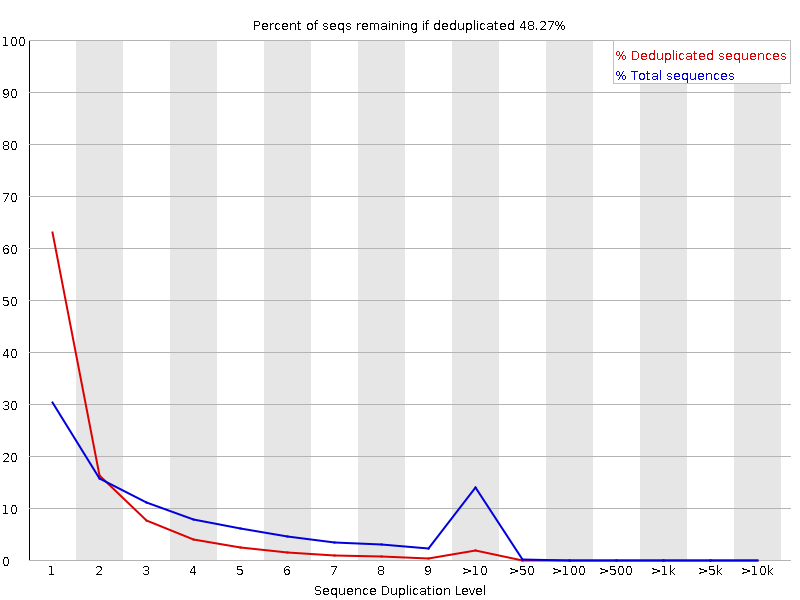
\includegraphics[width=\linewidth]{04-R1.qfilter_fastqc/Images/duplication_levels.png}
\caption{Sequence Duplication Levels: FAIL}
\end{subfigure}
\begin{subfigure}{0.45\linewidth}
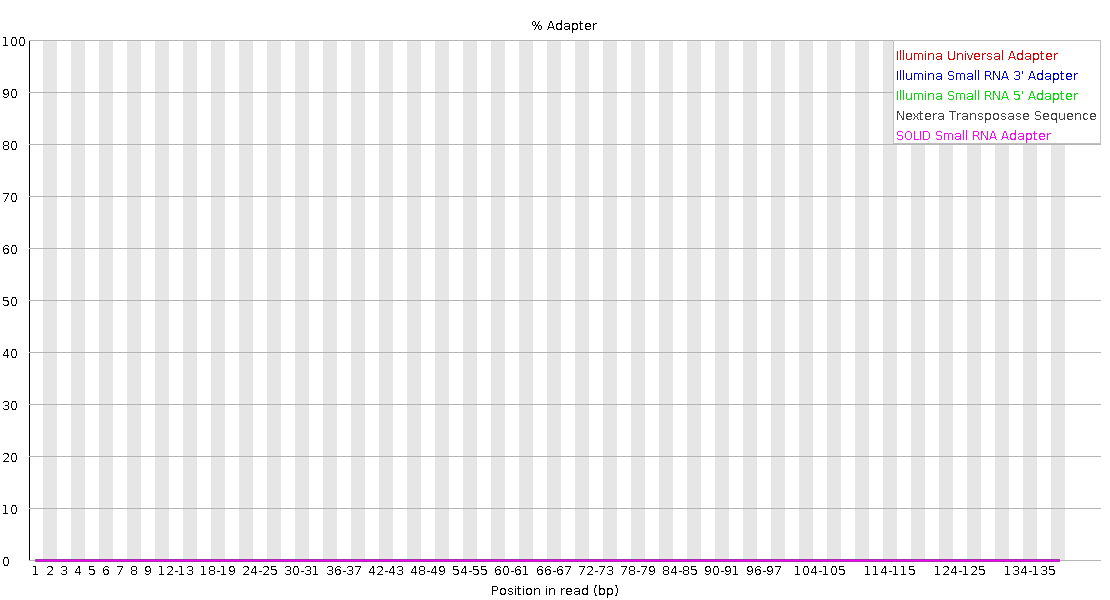
\includegraphics[width=\linewidth]{04-R1.qfilter_fastqc/Images/adapter_content.png}
\caption{Adapter content: PASS}
\end{subfigure}
\begin{subfigure}{0.45\linewidth}
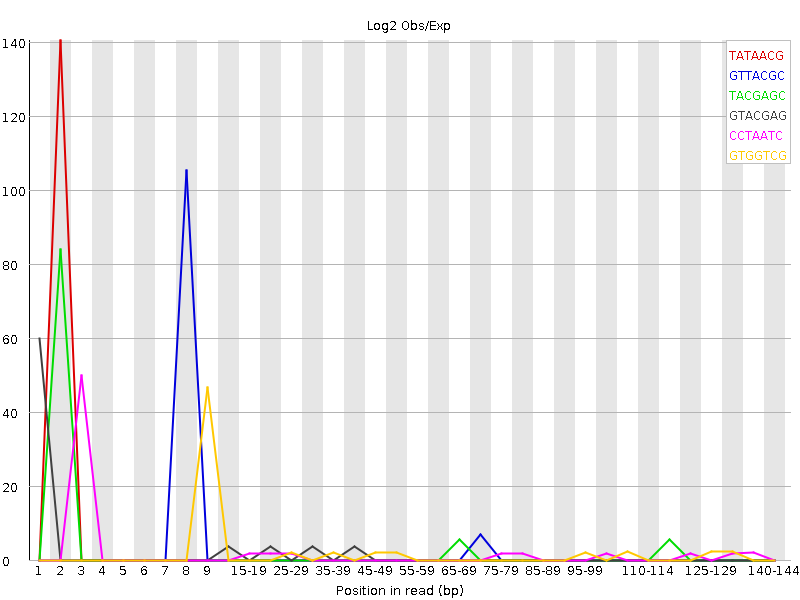
\includegraphics[width=\linewidth]{04-R1.qfilter_fastqc/Images/kmer_profiles.png}
\caption{Kmer content: WARN}
\end{subfigure}
\end{figure}


\end{document}